\documentclass[main.tex]{subfiles}

\begin{document}
\chapter{Literature Review}
\chaplabel{literatureReview}

\section{Navigation}
\subsection{Defining a Path Based on a Region}
\textbf{\color{red}{JONO CAN YOU TALK ABOUT DIFFERENT METHODS DO DEFINE A PATH BASED ON A REGION HERE, or maybe we dont even need to mention it, put in detailed design?}}

\subsection{Path Tracking}
\subsubsection{Geometric Path Tracking}
Geometric path tracking uses geometric relationships between a vehicle and a path to produce a control algorithm as a solution to the problem. Theories assume vehicles use the Ackermann method for steering so a simplified steering model can be used for geometric relationships. This reveals a relationship between the steering angle and the curvature that the non steering wheels will follow. Two of the most commonly used geometric vehicle methods are Pure Pursuit and the Stanley Method \parencite{snider2009}.

Pure Pursuit uses a path 'look-ahead' distance to measure the future error between the vehicle and the path in real time which can then be steered to and corrected for before it happens. \Figref{purePursuitGeom} is the geometry associated with Pure Pursuit at one point in time. It shows a goal point $(g_x, g_y)$ on the desired path at specified look-ahead distance $l_d$ in front of the vehicle. The steer angle is calculated based on an arc that would connect the centre of the non-steering axle to the goal point. When high curvatures are present in a path the controller may also begin to cut corners due to a look-ahead distance that would effectively skip this portion of the path. Constant lateral error on a path of constant curvature may also be experienced due to geometric controller characteristics which do not take into account the curvature of a path. However, Pure Pursuit provides a very robust tracking algorithm when discontinuous curvatures are present \parencite{snider2009}. In general, for more accurate tracking a short look-ahead distance should be used but will eventually can result in oscillation, for smoother tracking a long look-ahead distance should be used but will reduce precision \parencite{snider2009}.
\begin{figure}[ht]
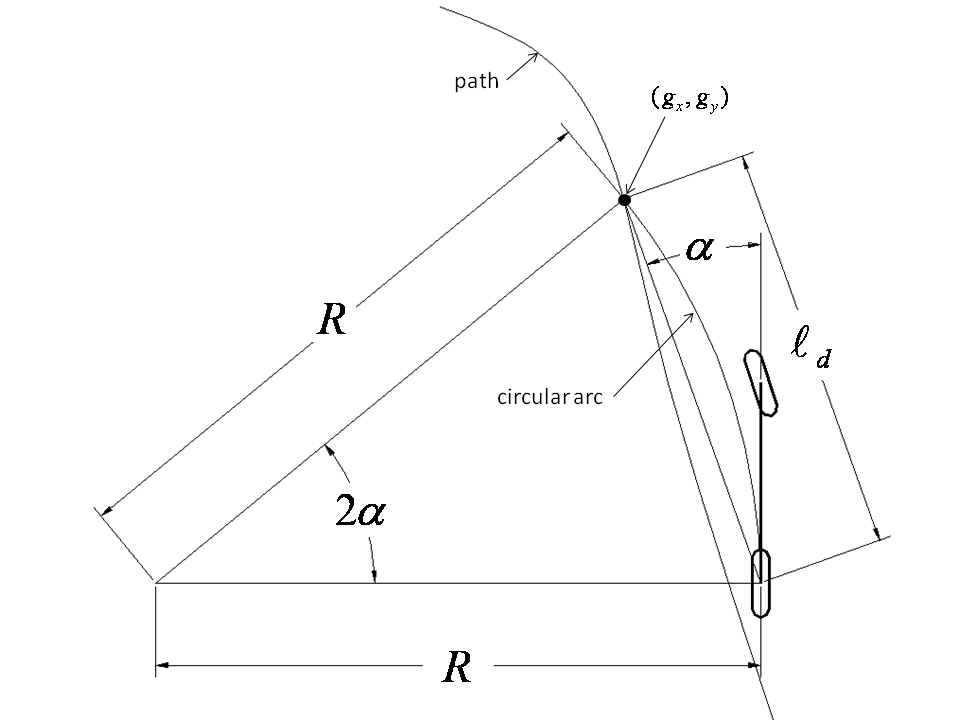
\includegraphics[width=0.6\textwidth]{3-LiteratureReview/purePursuitGoal.png}
\centering
\caption{Pure Pursuit Geometry \parencite{snider2009}} \figlabel{purePursuitGeom}
\end{figure}

The Stanley Model 
\begin{figure}[ht]
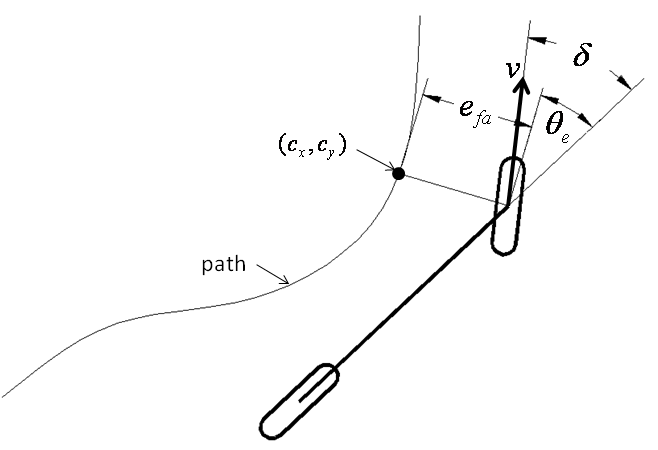
\includegraphics[width=0.5\textwidth]{3-LiteratureReview/stanleyMethod.png}
\centering
\caption{Stanley Method Geometry \parencite{snider2009}} \figlabel{stanleyGeom}
\end{figure}

Some limitations of geometric path tracking methods are related to the dynamics of a vehicle which are not present in the theory, namely the capabilities of a platform and its actuators. Due to this the method expects an instant response from elements such as the steering which is an issue when high path curvatures are present or when the curvature of the path suddenly changes. As a result the method cannot guarantee that the vehicle will follow a path as accurately as designed and at high speeds that vehicle may skid or tip \parencite{coulter1992}.

\subsection{Turning a Specified Angle}


\end{document}
